% !TEX program = xelatex
\documentclass[UTF8,zihao=-4,oneside,openany]{ctexbook}

% Shared style for the combined handout.  Section files keep standalone
% preambles for now, while the master document uses this single definition.
\usepackage[a4paper,top=20mm,bottom=22mm,left=19mm,right=19mm,headheight=24pt]{geometry}
\usepackage[table]{xcolor}
\usepackage{amsmath,amssymb,mathtools,bm}
\usepackage{siunitx}
\usepackage{booktabs,tabularx,array,multicol}
\usepackage{enumitem}
\usepackage{tikz}
\usetikzlibrary{arrows.meta,positioning,calc,angles,quotes,patterns}
\usepackage[most]{tcolorbox}
\usepackage{fancyhdr}
\usepackage{hyperref}

\definecolor{Ink}{HTML}{202326}
\definecolor{DeepBlue}{HTML}{294E69}
\definecolor{Blue}{HTML}{47687D}
\definecolor{PaleBlue}{HTML}{F3F5F6}
\definecolor{Gold}{HTML}{6E777D}
\definecolor{PaleGold}{HTML}{F6F6F5}
\definecolor{Green}{HTML}{5B6D76}
\definecolor{PaleGreen}{HTML}{F3F5F6}
\definecolor{Alert}{HTML}{666B6F}
\definecolor{PaleAlert}{HTML}{F6F6F6}
\definecolor{RuleGray}{HTML}{D3D7DA}
\definecolor{TextGray}{HTML}{61686D}
\definecolor{SoftGray}{HTML}{F6F6F6}

\color{Ink}
\sisetup{
  per-mode=symbol,
  inter-unit-product=\ensuremath{{}\cdot{}},
  exponent-product=\times
}

\hypersetup{
  colorlinks=true,
  linkcolor=DeepBlue,
  urlcolor=Blue,
  pdfsubject={高中物理竞赛一轮资料重排讲义},
  pdfauthor={物理竞赛一轮资料编写组}
}

\setlength{\parindent}{2em}
\setlength{\parskip}{0.25em}
\setlist{nosep,leftmargin=2em}
\setcounter{secnumdepth}{3}
\setcounter{tocdepth}{2}
\numberwithin{equation}{section}
\counterwithin{table}{section}
\allowdisplaybreaks[2]
\emergencystretch=2em

\ctexset{
  chapter={
    format=\raggedright\LARGE\bfseries\color{Ink},
    titleformat=\LARGE\bfseries\color{Ink},
    beforeskip=0pt,
    afterskip=18pt
  },
  section={
    format=\Large\bfseries\color{DeepBlue},
    beforeskip=1.8ex,
    afterskip=1.0ex
  },
  subsection={
    format=\large\bfseries\color{Ink},
    beforeskip=1.5ex,
    afterskip=0.8ex
  },
  subsubsection={format=\normalsize\bfseries\color{Ink}}
}

\pagestyle{fancy}
\fancyhf{}
\fancyhead[L]{\small\color{TextGray}高中物理竞赛一轮讲义}
\fancyhead[R]{\small\color{TextGray}第一章\quad 数学与物理工具}
\fancyfoot[C]{\small\color{TextGray}\thepage}
\renewcommand{\headrulewidth}{0.4pt}
\renewcommand{\headrule}{\hbox to\headwidth{\color{RuleGray}\leaders\hrule height \headrulewidth\hfill}}

\newcommand{\dimens}[1]{\operatorname{dim}\!\left(#1\right)}
\newcommand{\dd}{\mathop{}\!\mathrm{d}}
\newcommand{\vect}[1]{\bm{#1}}
\newcommand{\uvec}[1]{\hat{\vect{#1}}}
\newcommand{\e}{\mathrm e}
\newcommand{\order}[1]{\mathcal O\!\left(#1\right)}
\DeclareMathOperator{\proj}{proj}
\newcommand{\examplesource}[1]{%
  \par{\small\color{TextGray}题源：#1}\par
}

\newtcolorbox{goalbox}{
  enhanced,breakable,
  colback=PaleBlue,colframe=Blue,
  boxrule=0.7pt,arc=2mm,
  title={本节目标},fonttitle=\bfseries,
  coltitle=DeepBlue,
  attach boxed title to top left={xshift=5mm,yshift=-2mm},
  boxed title style={colback=white,colframe=Blue,boxrule=0.7pt,arc=1.5mm}
}

\newtcolorbox{sourcebox}{
  enhanced,breakable,
  colback=SoftGray,colframe=RuleGray,
  boxrule=0.5pt,arc=0mm,
  title={题源说明},fonttitle=\bfseries,
  coltitle=Ink,colbacktitle=SoftGray,
  borderline west={1.2pt}{0pt}{TextGray}
}

\newtcolorbox[auto counter,number within=section]{examplebox}[2][]{
  enhanced,breakable,
  colback=white,colframe=RuleGray,
  boxrule=0.5pt,arc=0mm,
  title={例题~\thetcbcounter\quad #2},fonttitle=\bfseries,
  coltitle=Ink,colbacktitle=PaleBlue,
  borderline west={1.4pt}{0pt}{DeepBlue},
  #1
}

\newtcolorbox{methodbox}[1]{
  enhanced,breakable,
  colback=PaleBlue,colframe=RuleGray,
  boxrule=0.5pt,arc=0mm,
  title={方法：#1},fonttitle=\bfseries,
  coltitle=Ink,colbacktitle=PaleBlue,
  borderline west={1.2pt}{0pt}{DeepBlue}
}

\newtcolorbox{warningbox}[1]{
  enhanced,breakable,
  colback=SoftGray,colframe=RuleGray,
  boxrule=0.5pt,arc=0mm,
  title={易错提醒：#1},fonttitle=\bfseries,
  coltitle=Ink,colbacktitle=SoftGray,
  borderline west={1.2pt}{0pt}{TextGray}
}

\newtcolorbox{extensionbox}[1]{
  enhanced,breakable,
  colback=PaleGold,colframe=Gold,
  boxrule=0.5pt,arc=0mm,
  title={拓展：#1},fonttitle=\bfseries,
  coltitle=Ink,colbacktitle=PaleGold,
  borderline west={1.2pt}{0pt}{DeepBlue}
}

\newtcolorbox{summarybox}{
  enhanced,breakable,
  colback=PaleBlue,colframe=DeepBlue,
  boxrule=0.9pt,arc=1.5mm,
  title={本节小结},fonttitle=\bfseries,
  coltitle=white,colbacktitle=DeepBlue
}

\newtcolorbox{exercisebox}[1]{
  enhanced,breakable,
  colback=white,colframe=RuleGray,
  boxrule=0.7pt,arc=1.5mm,
  title={#1},fonttitle=\bfseries,
  coltitle=DeepBlue,colbacktitle=PaleBlue
}

\tikzset{
  vector/.style={-{Latex[length=2.5mm]},very thick,draw=DeepBlue},
  component/.style={-{Latex[length=2.2mm]},thick,draw=TextGray},
  axis/.style={-{Latex[length=2mm]},thin,draw=TextGray},
  guide/.style={densely dashed,draw=TextGray},
  curve/.style={very thick,draw=DeepBlue},
  tangent/.style={thick,draw=TextGray},
  secant/.style={thick,draw=DeepBlue}
}

\usetikzlibrary{decorations.pathmorphing,intersections,patterns.meta}
\newcommand{\Needspace}[1]{%
  \par
  \ifdim\dimexpr\pagegoal-\pagetotal\relax<#1\relax
    \newpage
  \fi
}

\newif\ifwithsolutions
\ifdefined\NOSOLUTIONS
  \withsolutionsfalse
\else
  \withsolutionstrue
\fi

\ifwithsolutions
  \hypersetup{
    pdftitle={学而思物理竞赛一轮资料重排：第一章第二节 积分及其应用（含补写解答与解图）},
    pdfsubject={学而思物理竞赛一轮资料重排；正文与例题据原资料整理，解答与解图为后补},
    pdfauthor={原资料：学而思；重排与补写解答：物理竞赛一轮资料编写组}
  }
\else
  \hypersetup{
    pdftitle={学而思物理竞赛一轮资料重排：第一章第二节 积分及其应用},
    pdfsubject={学而思物理竞赛一轮资料原版重排；无解答版},
    pdfauthor={原资料：学而思；重排：物理竞赛一轮资料编写组}
  }
\fi

\fancyhead[R]{\small\color{TextGray}第一章\quad 微积分在物理当中的应用}
\renewcommand{\theequation}{\thechapter.\arabic{equation}}

\newtcolorbox{origexamplebox}[1]{
  enhanced,breakable,
  colback=white,colframe=RuleGray,
  boxrule=0.5pt,arc=0mm,
  title={#1},fonttitle=\bfseries,
  coltitle=Ink,colbacktitle=PaleBlue,
  borderline west={1.4pt}{0pt}{DeepBlue}
}

\NewDocumentEnvironment{xesolution}{+b}{%
  \ifwithsolutions
    \par\smallskip
    \begingroup\small
    \noindent{\bfseries\color{DeepBlue}解答}\quad #1
    \par\endgroup\medskip
  \fi
}{}

% TikZ figures redrawn from the source; annotations used only in solutions are
% drawn in the restrained blue accent of the common style.

\newcommand{\partitionDiagram}{%
\begin{center}
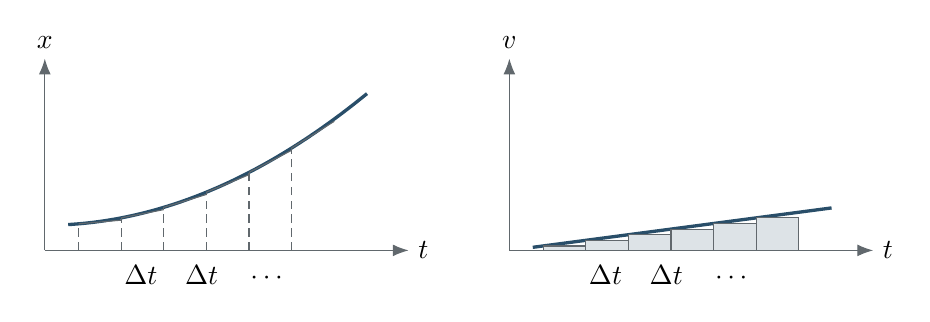
\begin{tikzpicture}[x=0.66cm,y=0.58cm,>=Latex]
  \begin{scope}
    \draw[axis] (0,0)--(7.0,0) node[right] {$t$};
    \draw[axis] (0,0)--(0,4.2) node[above] {$x$};
    \draw[curve,domain=0.45:6.2,smooth,variable=\t]
      plot ({\t},{0.55+0.075*\t*\t});
    \foreach \i in {1,...,6}{
      \pgfmathsetmacro{\xa}{0.65+0.82*(\i-1)}
      \pgfmathsetmacro{\xb}{0.65+0.82*\i}
      \pgfmathsetmacro{\ya}{0.55+0.075*\xa*\xa}
      \pgfmathsetmacro{\slope}{0.15*\xa}
      \draw[TextGray] (\xa,\ya)--(\xb,{\ya+\slope*(\xb-\xa)});
      \draw[guide] (\xa,0)--(\xa,\ya);
    }
    \node[below] at (3.1,-0.12) {$\Delta t\quad\Delta t\quad\cdots$};
  \end{scope}
  \begin{scope}[xshift=5.9cm]
    \draw[axis] (0,0)--(7.0,0) node[right] {$t$};
    \draw[axis] (0,0)--(0,4.2) node[above] {$v$};
    \draw[curve,domain=0.45:6.2,smooth,variable=\t]
      plot ({\t},{0.15*\t});
    \foreach \i in {1,...,6}{
      \pgfmathsetmacro{\xa}{0.65+0.82*(\i-1)}
      \pgfmathsetmacro{\xb}{0.65+0.82*\i}
      \pgfmathsetmacro{\ya}{0.15*\xa}
      \draw[fill=DeepBlue!16,draw=TextGray] (\xa,0) rectangle (\xb,\ya);
    }
    \node[below] at (3.1,-0.12) {$\Delta t\quad\Delta t\quad\cdots$};
  \end{scope}
\end{tikzpicture}

{\small\color{TextGray}图 1.5\quad 同一运动的 $x(t)$ 与 $v(t)=x'(t)$：左图的切线增量等于右图对应矩形的面积，均为 $v(t_i)\Delta t$。}
\end{center}}

\newcommand{\integralDiagram}{%
\begin{center}
\begin{tikzpicture}[x=0.9cm,y=0.7cm,>=Latex]
  \draw[axis] (0,0)--(7.2,0) node[right] {$x$};
  \draw[axis] (0,0)--(0,4.1) node[above] {$y$};
  \pgfmathdeclarefunction{areaheight}{1}{\pgfmathparse{3.1-.23*(##1-3.2)^2}}
  \fill[DeepBlue!14] (1.1,0)
    -- plot[domain=1.1:5.45,samples=90] (\x,{areaheight(\x)})
    --(5.45,0)--cycle;
  \draw[curve,domain=.35:6.2,samples=100] plot (\x,{areaheight(\x)});
  \draw[thick] (1.1,0)--(1.1,{areaheight(1.1)})
    (5.45,0)--(5.45,{areaheight(5.45)});
  \node[below] at (1.1,0) {$a$}; \node[below] at (5.45,0) {$b$};
  \node[above] at (3.2,3.1) {$f(x)$};
  \node[align=center,anchor=north] at (3.45,-.65)
    {$\displaystyle \frac{\dd F}{\dd x}=f(x)$\\[2pt]
     $\displaystyle \int_a^b f(x)\dd x=F(b)-F(a)$};
\end{tikzpicture}

{\small\color{TextGray}图 1.6\quad 积分的代数和几何意义}
\end{center}}

\newcommand{\areaLineDiagram}{%
\begin{center}
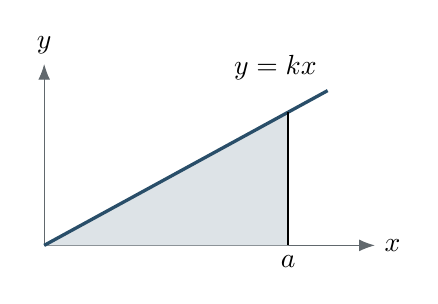
\begin{tikzpicture}[x=1cm,y=0.72cm,>=Latex]
  \draw[axis] (0,0)--(4.2,0) node[right] {$x$};
  \draw[axis] (0,0)--(0,3.2) node[above] {$y$};
  \fill[DeepBlue!16] (0,0)--(3.1,0)--(3.1,2.35)--cycle;
  \draw[curve] (0,0)--(3.6,2.73) node[above left] {$y=kx$};
  \draw[thick] (3.1,0)--(3.1,2.35);
  \node[below] at (3.1,0) {$a$};
\end{tikzpicture}
\end{center}}

\newcommand{\areaParabolaDiagram}{%
\begin{center}
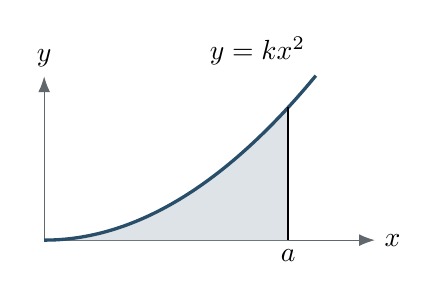
\begin{tikzpicture}[x=1cm,y=0.65cm,>=Latex]
  \draw[axis] (0,0)--(4.2,0) node[right] {$x$};
  \draw[axis] (0,0)--(0,3.2) node[above] {$y$};
  \fill[DeepBlue!16] (0,0) plot[domain=0:3.1,smooth,variable=\x]
    ({\x},{0.27*\x*\x}) --(3.1,0)--cycle;
  \draw[curve,domain=0:3.45,smooth,variable=\x]
    plot ({\x},{0.27*\x*\x}) node[above left] {$y=kx^2$};
  \draw[thick] (3.1,0)--(3.1,{0.27*3.1*3.1});
  \node[below] at (3.1,0) {$a$};
\end{tikzpicture}
\end{center}}

\newcommand{\circlePartitionsDiagram}{%
\begin{center}
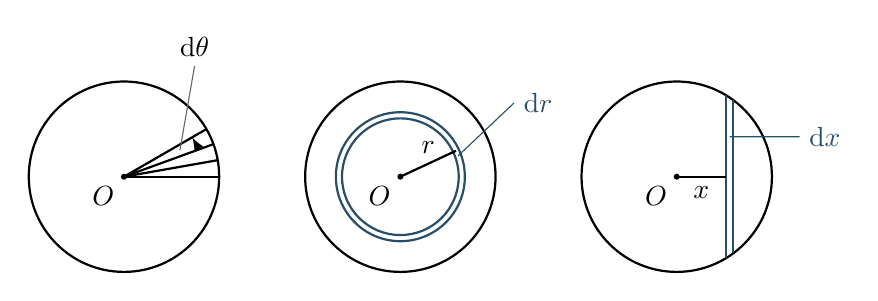
\begin{tikzpicture}[scale=0.78,>=Latex]
  \begin{scope}
    \draw[thick] (0,0) circle (1.55);
    \foreach \a in {0,10,20,30}{\draw[thick] (0,0)--(\a:1.55);}
    \coordinate (Oa) at (0,0);
    \coordinate (A20) at (20:1);
    \coordinate (A30) at (30:1);
    \draw pic[draw,->,angle radius=10mm] {angle=A20--Oa--A30};
    \node (anglelabel) at (1.15,2.12) {$\dd\theta$};
    \draw[TextGray,thin] (anglelabel.south)--(.91,.43);
    \fill (0,0) circle (1.4pt) node[below left] {$O$};
  \end{scope}
  \begin{scope}[xshift=4.5cm]
    \draw[thick] (0,0) circle (1.55);
    \draw[DeepBlue,thick] (0,0) circle (0.95);
    \draw[DeepBlue,thick] (0,0) circle (1.05);
    \draw[thick] (0,0)--(25:1.0) node[midway,above] {$r$};
    \node[DeepBlue,anchor=west] (drlabel) at (1.85,1.20) {$\dd r$};
    \draw[DeepBlue,thin] (drlabel.west)--(.94,.34);
    \fill (0,0) circle (1.4pt) node[below left] {$O$};
  \end{scope}
  \begin{scope}[xshift=9.0cm]
    \draw[thick] (0,0) circle (1.55);
    \draw[DeepBlue,thick] (0.8,-1.33)--(0.8,1.33);
    \draw[DeepBlue,thick] (0.92,-1.25)--(0.92,1.25);
    \draw[thick] (0,0)--(0.8,0) node[midway,below] {$x$};
    \node[DeepBlue,anchor=west] (dxlabel) at (2.0,.65) {$\dd x$};
    \draw[DeepBlue,thin] (dxlabel.west)--(.86,.65);
    \fill (0,0) circle (1.4pt) node[below left] {$O$};
  \end{scope}
\end{tikzpicture}
\end{center}}

\newcommand{\massElementsDiagram}{%
\begin{center}
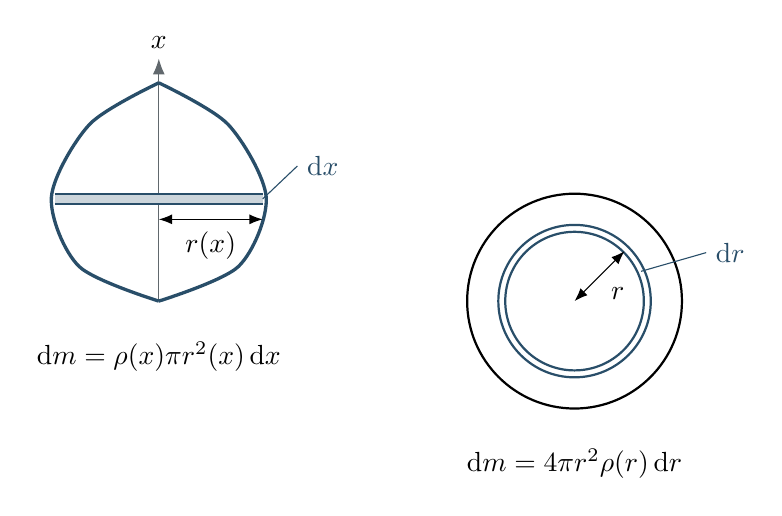
\begin{tikzpicture}[scale=0.88,>=Latex]
  \begin{scope}
    \draw[axis] (0,0)--(0,3.5) node[above] {$x$};
    \draw[curve] plot[smooth] coordinates {(0,0) (1.15,0.5) (1.55,1.5) (1.0,2.55) (0,3.15)};
    \draw[curve] plot[smooth] coordinates {(0,0) (-1.15,0.5) (-1.55,1.5) (-1.0,2.55) (0,3.15)};
    \fill[DeepBlue!24] (-1.5,1.4) rectangle (1.5,1.55);
    \draw[DeepBlue,thick] (-1.5,1.4)--(1.5,1.4) (-1.5,1.55)--(1.5,1.55);
    \draw[<->] (0,1.18)--(1.5,1.18);
    \node[below=1pt] at (0.75,1.18) {$r(x)$};
    \node[DeepBlue,anchor=west] (dxlabel) at (2.0,1.95) {$\dd x$};
    \draw[DeepBlue,thin] (dxlabel.west)--(1.5,1.475);
    \node[below] at (0,-0.45) {$\dd m=\rho(x)\pi r^2(x)\dd x$};
  \end{scope}
  \begin{scope}[xshift=6.0cm]
    \draw[thick] (0,0) circle (1.55);
    \draw[DeepBlue,thick] (0,0) circle (1.0);
    \draw[DeepBlue,thick] (0,0) circle (1.1);
    \draw[<->] (0,0)--(0.72,0.72);
    \node[below right=1pt] at (0.36,0.36) {$r$};
    \node[DeepBlue,anchor=west] (drlabel) at (1.90,.70) {$\dd r$};
    \draw[DeepBlue,thin] (drlabel.west)--(.96,.43);
    \node[below] at (0,-2.0) {$\dd m=4\pi r^2\rho(r)\dd r$};
  \end{scope}
\end{tikzpicture}
\end{center}}

\newcommand{\pvWorkDiagram}{%
\begin{center}
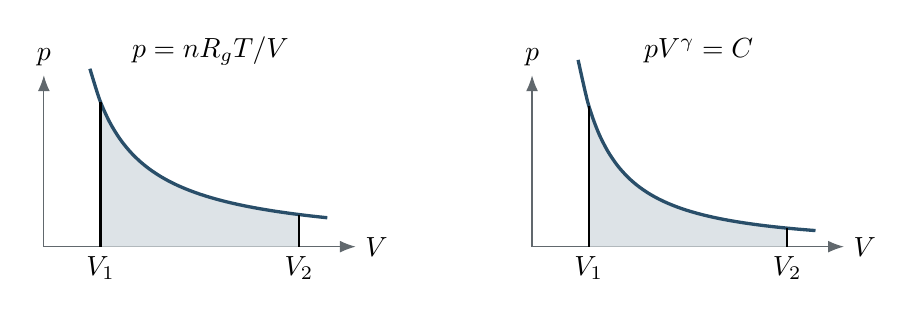
\begin{tikzpicture}[x=0.9cm,y=0.68cm,>=Latex]
  \begin{scope}
    \draw[axis] (0,0)--(4.4,0) node[right] {$V$};
    \draw[axis] (0,0)--(0,3.2) node[above] {$p$};
    \fill[DeepBlue!16] (0.8,0)
      -- plot[domain=0.8:3.6,smooth,variable=\x] ({\x},{2.16/\x})--(3.6,0)--cycle;
    \draw[curve,domain=0.65:4.0,smooth,variable=\x]
      plot ({\x},{2.16/\x});
    \node at (2.35,3.65) {$p=nR_gT/V$};
    \draw[thick] (0.8,0)--(0.8,2.7) (3.6,0)--(3.6,0.6);
    \node[below] at (0.8,0) {$V_1$}; \node[below] at (3.6,0) {$V_2$};
  \end{scope}
  \begin{scope}[xshift=6.2cm]
    \draw[axis] (0,0)--(4.4,0) node[right] {$V$};
    \draw[axis] (0,0)--(0,3.2) node[above] {$p$};
    \fill[DeepBlue!16] (0.8,0)
      -- plot[domain=0.8:3.6,smooth,variable=\x] ({\x},{1.95/(\x^1.35)})--(3.6,0)--cycle;
    \draw[curve,domain=0.65:4.0,smooth,variable=\x]
      plot ({\x},{1.95/(\x^1.35)});
    \node at (2.35,3.65) {$pV^\gamma=C$};
    \draw[thick] (0.8,0)--(0.8,{1.95/(.8^1.35)})
      (3.6,0)--(3.6,{1.95/(3.6^1.35)});
    \node[below] at (0.8,0) {$V_1$}; \node[below] at (3.6,0) {$V_2$};
  \end{scope}
\end{tikzpicture}
\end{center}}

\newcommand{\radialFallDiagram}{%
\begin{center}
\begin{tikzpicture}[scale=0.9,>=Latex]
  \fill (0,0) circle (4pt) node[above left=2pt] {$A(M)$};
  \draw[axis] (0,0)--(5.35,0) node[right] {径向坐标};
  \draw[DeepBlue,dashed] (4.75,0) circle (3.0pt);
  \node[above=8pt,DeepBlue] at (4.75,0) {$m(0)$};
  \fill[DeepBlue] (3.25,0) circle (2.5pt);
  \node[below left=3pt,DeepBlue] at (3.25,0) {$m(t)$};
  \draw[vector] (3.1,0.68)--(2.05,0.68) node[midway,above] {$\vec v$};
  \draw[<->] (0,-0.72)--(3.25,-0.72);
  \node[below=1pt] at (1.63,-0.72) {$r$};
  \draw[<->,TextGray] (0,-1.28)--(4.75,-1.28);
  \node[below=1pt,TextGray] at (2.38,-1.28) {$r_0$};
  \draw[guide] (3.25,-0.9)--(3.25,0);
  \draw[guide] (4.75,-1.44)--(4.75,0);
\end{tikzpicture}
\end{center}}

\newcommand{\arcLengthDiagram}{%
\begin{center}
\begin{tikzpicture}[x=1cm,y=0.72cm,>=Latex]
  \draw[axis] (0,0)--(5.8,0) node[right] {$x$};
  \draw[axis] (0,0)--(0,3.5) node[above] {$y$};
  \draw[curve,domain=.55:4.6,samples=80] plot (\x,{1.4+.27*(\x-2.3)^2});
  \draw[thick] (1.2,0)--(1.2,{1.4+.27*(1.2-2.3)^2})
    (4.35,0)--(4.35,{1.4+.27*(4.35-2.3)^2});
  \node[below] at (1.2,0) {$x_1$}; \node[below] at (4.35,0) {$x_2$};
  \coordinate (P) at (7.0,1.2);
  \coordinate (H) at (9.0,1.2);
  \coordinate (Q) at (9.0,{1.2+2*.54*(3.7-2.3)});
  \draw[guide] (3.7,{1.4+.27*(3.7-2.3)^2})--(6.7,2.9);
  \node[TextGray,above] at (8,3.2) {局部切线三角形};
  \draw[DeepBlue,very thick] (P)--(Q) node[midway,above left] {$\dd s$};
  \draw[component] (P)--(H) node[midway,below] {$\dd x$};
  \draw[component] (H)--(Q) node[midway,right] {$\dd y$};
  \draw[TextGray,line width=.45pt] ($(H)+(-.13,0)$)--($(H)+(-.13,.13)$)--($(H)+(0,.13)$);
  \node[above left] at (4.55,2.78) {$y(x)$};
\end{tikzpicture}
\end{center}}

\newcommand{\trackTimeDiagram}{%
\begin{center}
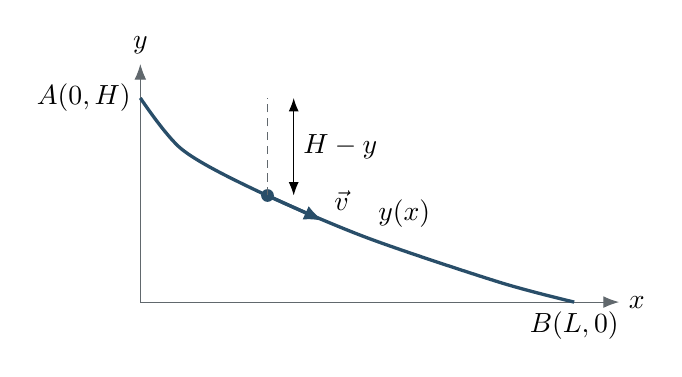
\begin{tikzpicture}[x=0.95cm,y=0.72cm,>=Latex]
  \draw[axis] (0,0)--(6.4,0) node[right] {$x$};
  \draw[axis] (0,0)--(0,4.2) node[above] {$y$};
  \draw[curve] plot[smooth] coordinates {(0,3.6) (0.55,2.7) (1.5,2.0) (3.0,1.15) (4.8,0.35) (5.8,0)};
  \fill[DeepBlue] (1.7,1.88) circle (2.3pt);
  \draw[vector] (1.7,1.88)--++(0.75,-0.45) node[above right] {$\vec v$};
  \draw[guide] (1.7,1.88)--(1.7,3.6);
  \draw[<->] (2.05,1.88)--node[right] {$H-y$}(2.05,3.6);
  \node[left] at (0,3.6) {$A(0,H)$};
  \node[below] at (5.8,0) {$B(L,0)$};
  \node[above right] at (3.05,1.15) {$y(x)$};
\end{tikzpicture}
\end{center}}

\newcommand{\trackTimeSolutionDiagram}{%
\begin{center}
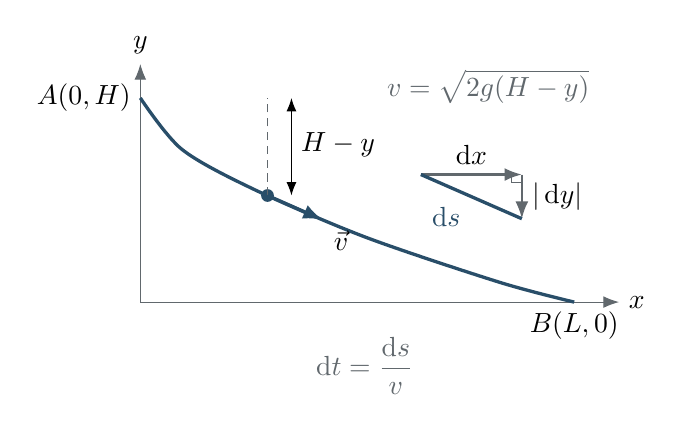
\begin{tikzpicture}[x=0.95cm,y=0.72cm,>=Latex]
  \draw[axis] (0,0)--(6.4,0) node[right] {$x$};
  \draw[axis] (0,0)--(0,4.2) node[above] {$y$};
  \draw[curve] plot[smooth] coordinates
    {(0,3.6) (0.55,2.7) (1.5,2.0) (3.0,1.15) (4.8,0.35) (5.8,0)};
  \coordinate (P) at (1.70,1.88);
  \fill[DeepBlue] (P) circle (2.3pt);
  \draw[guide] (P)--(1.70,3.6);
  \draw[<->] (2.02,1.88)--(2.02,3.6);
  \node[right] at (2.02,2.78) {$H-y$};
  \draw[vector] (P)--++(0.74,-0.43) node[below right] {$\vec v$};
  \node[left] at (0,3.6) {$A(0,H)$};
  \node[below] at (5.8,0) {$B(L,0)$};
  \node[align=left,TextGray] at (4.65,3.8)
    {$\displaystyle v=\sqrt{2g(H-y)}$};
  \node[anchor=north,TextGray] at (3.0,-.45)
    {$\displaystyle \dd t=\frac{\dd s}{v}$};
  \begin{scope}[shift={(3.75,2.25)}]
    \coordinate (U) at (0,0);
    \coordinate (V) at (1.35,0);
    \coordinate (W) at (1.35,-0.78);
    \draw[component] (U)--(V) node[midway,above] {$\dd x$};
    \draw[component] (V)--(W) node[midway,right] {$|\dd y|$};
    \draw[DeepBlue,very thick] (U)--(W) node[midway,below left] {$\dd s$};
    \draw[TextGray,line width=.45pt]
      ($(V)+(-.14,0)$)--($(V)+(-.14,-.14)$)--($(V)+(0,-.14)$);
  \end{scope}
\end{tikzpicture}
\end{center}}


\begin{document}
\pagenumbering{arabic}
\setcounter{page}{1}
\setcounter{chapter}{1}
\setcounter{section}{1}

\section{积分及其应用}
\setcounter{equation}{12}

回到运动学中，假设一艘船沿给定航线行驶。规定一个正方向后，为了确定船的位置，需要知道
它相对港口的带符号位移。船员能够记录船在不同时刻沿航线的速度，并据此推断当前位置。
如果船始终作匀速直线运动，只需用速度乘时间即可得到位移；但实际速度会不断变化，因而
需要由速度随时间的函数计算变速运动中的位移。若另求航程，才应把各段路程作为正量相加。

\partitionDiagram

把时间分成许多小段。设物体在时刻 $t$ 的速度为 $v(t)$，若时间段 $\Delta t$ 足够小，
可近似认为速度在这段时间内不变，于是从 $t$ 到 $t+\Delta t$ 的位移近似为
\begin{equation}
 \Delta x\simeq v(t)\Delta t.
\end{equation}
在 $x$--$t$ 图像上，这段位移是以 $v(t)$ 为斜率的短直线段在竖直方向的投影；在
$v$--$t$ 图像上，它是宽为 $\Delta t$、高为 $v(t)$ 的窄矩形面积。把所有小段相加，
并令 $\Delta t$ 趋于零，折线趋近真实的 $x(t)$ 曲线，矩形面积之和趋近 $v$--$t$
曲线下的面积。

已知位置函数时，速度由
\begin{equation}
 v(t)=\frac{\dd x}{\dd t}(t)
\end{equation}
给出。现在要解决的是它的逆问题：已知一条曲线各点的导数，怎样求曲线本身。解决这类
问题的方法就是积分。

若函数 $F(x)$ 的导数为 $f(x)$，则称 $F(x)$ 是 $f(x)$ 的一个原函数，并写成
\begin{equation}
 \int f(x)\dd x=F(x)+C,
\end{equation}
这称为 $f(x)$ 的不定积分（indefinite integration），其中 $f(x)$ 为被积函数，$x$ 为
积分变量，$C$ 为积分常数。若原函数已知，则 $f(x)$ 在 $x_1$ 到 $x_2$ 之间的定积分为
\begin{equation}
 \int_{x_1}^{x_2}f(x)\dd x
 =\left.F(x)\right|_{x_1}^{x_2}=F(x_2)-F(x_1).
\end{equation}

\integralDiagram

积分可以处理曲线面积、复杂形体体积以及许多连续求和问题。基本思想是把复杂对象分割
成简单的小对象，先算出每个小对象的相应量，再在小对象趋于无穷小时把它们积分起来。
积分的线性规律为
\begin{equation}
 \int af(x)\dd x=a\int f(x)\dd x,
\end{equation}
\begin{equation}
 \int[f(x)+g(x)]\dd x
 =\int f(x)\dd x+\int g(x)\dd x.
\end{equation}

\Needspace{0.32\textheight}
\subsection{定积分的方向、运算与检验}

前述分割求和给出了定积分。它在 $v$--$t$ 图上表示有向面积：横轴下方的部分给负位移，而路程应对速率 $|v|$ 积分。类似地，
密度不均匀细棒的质量为 $m=\int\lambda(x)\dd x$，变力做功为
$W=\int\vec F\cdot\dd\vec r$，积分的共同思想都是“局部近似简单、整体取极限求和”。

若 $F'(x)=f(x)$，则
\[
 \int_a^b f(x)\,\dd x=F(b)-F(a).
\]
积分上限、下限和积分变量缺一不可；换元时微分和边界必须同时变换。分部积分
\[
 \int_a^b u\,\dd v=[uv]_a^b-\int_a^b v\,\dd u
\]
来自乘积求导法则，适于含对数、反三角函数或两个不同类型函数乘积的积分。结果求出后可通过
求导核对原函数，并用量纲和边界极限检查物理答案。

\subsection{积分建立物理量的空间分布}

连续分布的质心坐标满足
\[
 x_C=\frac1M\int x\,\dd m.
\]
关键是先把质量元写成合适坐标的函数，如细线 $\dd m=\lambda\dd l$、薄片
$\dd m=\sigma\dd S$、立体 $\dd m=\rho\dd V$。转动惯量
$I=\int r_\perp^2\dd m$ 同样依赖转轴到质量元的垂直距离。选择对称坐标后，许多奇函数部分积分为零；
在结果中保留这种对称性，比从一开始展开全部坐标更简洁。

微分方程把“局部变化规律”还原成运动。若 $m\dot v=F(v)$，可写成
$\dd v/F(v)=\dd t/m$ 再积分；更一般的 $F(v,t)$ 只有在它能够分解为速度函数与时间函数的乘积时才能分离变量。
由 $v\dd v/\dd x=a$ 可在不显含时间的问题中把二阶运动方程降阶。
积分常数由初始条件确定，不能因只求到一个原函数而省略。遇到分段力或分段约束时，应在每一段
分别积分，并在转换时刻用位置、速度的连续性或冲量条件衔接。

积分也能给出曲线长度、面积和体积。平面极坐标的一般面积元为
$\dd S=r\dd r\dd\theta$，柱坐标体积元为 $\dd V=r\dd r\dd\theta\dd z$；这些微元中的几何因子
不是记号装饰，而是坐标网格随位置伸缩的结果。若区域从原点延伸到边界 $r=R(\theta)$，先对半径积分才得到
$\int_0^{R(\theta)}r\dd r\dd\theta=\tfrac12R^2(\theta)\dd\theta$；后者是微小扇形面积，不是一般面积元。
先画出被积区域、再确定积分次序，能够避免漏算或重复。

\subsection{近似求积与物理积分的检查}

有些积分没有初等原函数，但定积分仍然有清楚的物理意义。可以把区间划分为小段，用矩形、梯形或
中点值近似每段面积；分割越细，数值和越接近真实积分。实验数据本来就是离散的，此时
\[
 \int_{t_1}^{t_2}F(t)\,\dd t
 \simeq\sum_i\frac{F_i+F_{i+1}}2(t_{i+1}-t_i)
\]
可直接由测得的力—时间数据估计冲量。数值积分给出的是近似值，应同时说明时间步长和误差怎样随
分割改变，而不能把计算器输出的许多小数位都当成有效数字。

广义积分还要求检查端点或无穷远是否收敛。例如总质量
$M=\int_0^\infty\lambda(x)\dd x$ 只有在密度衰减足够快时才有限；势能或电势把无穷远取作零点时，
也隐含了相应积分收敛。若积分发散，往往表示理想化模型不能延伸到无限远，而不是简单地说物理量
“等于无穷”。无限长导线、无限大平面等模型通常只能可靠给出场强或两个有限点之间的势差。

含参数的积分能够表示一族物理状态。若积分区间固定并满足适当光滑条件，可在积分号下求导：
\[
 \frac{\dd}{\dd a}\int_{x_1}^{x_2}f(x,a)\,\dd x
 =\int_{x_1}^{x_2}\frac{\partial f}{\partial a}\,\dd x.
\]
这个方法可把难积分转化为较容易的积分，再对参数积分回来；积分常数则由某个易求的参数值确定。
若上下限也依赖参数，还要加上端点移动产生的边界项。

任何物理积分至少应通过三项检查：被积式乘微元的量纲是否正确，改变积分方向时符号是否合理，
以及在均匀分布、恒力或恒速极限下能否退化为熟悉的初等公式。先写清微元代表什么，再写积分限，
往往比先套积分表更能避免错误。


\begin{origexamplebox}{例 1.17}
设 $a>0,k>0$。计算通过坐标原点的直线 $f(x)=kx$ 在 $x=0$ 到 $x=a$ 之间与横轴所围成的几何面积。
\areaLineDiagram
\end{origexamplebox}

\begin{xesolution}
把区间 $[0,a]$ 分成许多宽为 $\dd x$ 的小段，每个窄条的面积为
\[
 \dd S=f(x)\dd x=kx\dd x.
\]
将它们相加：
\[
 S=\int_0^a kx\dd x
 =\left.\frac12kx^2\right|_0^a
 =\boxed{\frac12ka^2}.
\]
这正是底为 $a$、高为 $ka$ 的三角形面积 $\frac12a\cdot ka$。
\end{xesolution}

\Needspace{0.32\textheight}
\begin{origexamplebox}{例 1.18}
设 $a>0,k>0$。计算抛物线 $f(x)=kx^2$ 在 $x=0$ 到 $x=a$ 之间与横轴所围成的几何面积。
\areaParabolaDiagram
\end{origexamplebox}

\begin{xesolution}
取宽为 $\dd x$ 的竖直窄条，其面积元为
\[
 \dd S=kx^2\dd x.
\]
因此
\[
 S=\int_0^a kx^2\dd x
 =\left.\frac{kx^3}{3}\right|_0^a
 =\boxed{\frac13ka^3}.
\]
若以外接矩形面积 $a\cdot ka^2=ka^3$ 作比较，抛物线下的面积恰为它的三分之一。
\end{xesolution}

\Needspace{0.42\textheight}
\begin{origexamplebox}{例 1.19}
把下列计算圆面积的分割思路用积分表示出来并计算圆的面积，与熟悉的公式
$S=\pi R^2$ 比较。
\begin{enumerate}[label=(\alph*),leftmargin=2.2em]
 \item 从圆心出发把圆分成许多扇形，每个扇形的顶角为 $\dd\theta$；
 \item 把圆分成许多厚度为 $\dd r$ 的圆环，每个圆环的内半径为 $r$；
 \item 把圆切成许多矩形，每个矩形到圆心的距离为 $x$，宽为 $\dd x$。
\end{enumerate}
\circlePartitionsDiagram
\end{origexamplebox}

\begin{xesolution}
三种分割方式都在计算同一个圆面积，只是所选面积元不同。

\textbf{(a) 扇形分割。}\quad 半径为 $R$、圆心角为 $\dd\theta$ 的小扇形面积为
\[
 \dd S=\frac12R^2\dd\theta.
\]
绕圆一周：
\[
 S=\int_0^{2\pi}\frac12R^2\dd\theta
 =\boxed{\pi R^2}.
\]

\textbf{(b) 圆环分割。}\quad 半径为 $r$、厚度为 $\dd r$ 的薄圆环可近似展开成长为
$2\pi r$、宽为 $\dd r$ 的矩形：
\[
 \dd S=2\pi r\dd r,
 \qquad
 S=\int_0^R2\pi r\dd r=\boxed{\pi R^2}.
\]

\textbf{(c) 竖条分割。}\quad 距圆心横坐标为 $x$ 的竖条，其高度由
$x^2+y^2=R^2$ 给出：
\[
 h(x)=2\sqrt{R^2-x^2}.
\]
所以
\[
 S=\int_{-R}^{R}2\sqrt{R^2-x^2}\dd x
 =4\int_0^R\sqrt{R^2-x^2}\dd x.
\]
令 $x=R\sin\phi$，$\dd x=R\cos\phi\dd\phi$：
\[
 S=4R^2\int_0^{\pi/2}\cos^2\phi\dd\phi
 =4R^2\cdot\frac\pi4
 =\boxed{\pi R^2}.
\]
三种积分都得到熟悉的圆面积公式。
\end{xesolution}

\begin{origexamplebox}{例 1.20}
利用积分证明圆锥体体积是同底等高圆柱体积的 $1/3$。
\end{origexamplebox}

\begin{xesolution}
设圆锥高为 $H$、底面半径为 $R$。从锥顶起沿轴线建立坐标 $x$，在 $x$ 处取厚度为
$\dd x$ 的圆盘。由相似三角形
\[
 r(x)=\frac{R}{H}x.
\]
圆盘体积元为
\[
 \dd V=\pi r^2(x)\dd x
 =\pi\frac{R^2}{H^2}x^2\dd x.
\]
从锥顶累加到底面：
\[
 V=\int_0^H\pi\frac{R^2}{H^2}x^2\dd x
 =\pi\frac{R^2}{H^2}\cdot\frac{H^3}{3}
 =\boxed{\frac13\pi R^2H}.
\]
同底等高圆柱体积为 $\pi R^2H$，故圆锥体积恰为其三分之一。
\end{xesolution}

在物理中经常会遇到复杂的求和过程。若一个物理量发生变化，与它相关的量也随之改变，
直接求和往往并不现实；但把变化过程分成无穷多足够小的部分时，各小段中的物理量变化
通常可以近似表达。

例如物体在某时刻速度为 $v$，在无限小时间 $\dd t$ 内可近似看作匀速运动：
\begin{equation}
 \Delta x\simeq v(t)\Delta t,
\end{equation}
在 $\Delta t\to0$ 的极限下写成
\begin{equation}
 \dd x=v\dd t.
\end{equation}
已知 $v(t)$ 时，从 $t_1$ 到 $t_2$ 的位移为
\begin{equation}
 x(t_2)-x(t_1)=\int_{t_1}^{t_2}v(t)\dd t.
\end{equation}
这里得到的是带符号的位移；若要求路程，应在速度变号处分段积分 $|v(t)|$。

又如某物体的热容量随温度变化为 $C(T)$，在小温区 $\Delta T$ 内吸收的热量近似为
\begin{equation}
 \Delta Q\simeq C(T)\Delta T.
\end{equation}
取极限得 $\dd Q=C(T)\dd T$，所以物体从 $T_1$ 升温至 $T_2$ 所需热量为
\begin{equation}
 Q=\int_{T_1}^{T_2}C(T)\dd T.
\end{equation}

\begin{origexamplebox}{例 1.21}
利用积分写出下列两个物体质量的表达式：
\begin{enumerate}[label=(\alph*),leftmargin=2.2em]
 \item 轴对称物体的底部为 $x=0$、顶部为 $x=H$，半径随 $x$ 的关系为 $r(x)$，
 密度随高度的关系为 $\rho(x)$；
 \item 半径为 $R$ 的球对称物体，密度与距球心距离 $r$ 的关系由函数 $\rho(r)$ 给出。
\end{enumerate}
\end{origexamplebox}

\begin{xesolution}
质量元总是 $\dd m=\rho\dd V$，关键在于按对称性选择体积元。

\textbf{(a)} 在高度 $x$ 处取厚度 $\dd x$ 的薄圆盘：
\[
 \dd V=\pi r^2(x)\dd x,
 \qquad
 \dd m=\rho(x)\pi r^2(x)\dd x.
\]
所以
\[
 \boxed{M=\int_0^H\rho(x)\pi r^2(x)\dd x}.
\]

\textbf{(b)} 在距球心 $r$ 处取厚度 $\dd r$ 的薄球壳，其体积元为
$4\pi r^2\dd r$，故
\[
 \boxed{M=4\pi\int_0^R\rho(r)r^2\dd r}.
\]
\massElementsDiagram
两个式子的上下限都从对称中心或底部开始，直到物体边界；量纲均为
$[\rho][\text{体积}]=[\text{质量}]$。
\end{xesolution}

\Needspace{0.38\textheight}
\begin{origexamplebox}{例 1.22}
一维运动中，外力与物体位置的关系为 $F(x)$。物体从 $x_1$ 运动到 $x_2$ 时，外力的功为
\[
 W_{12}=\int_{x_1}^{x_2}F(x)\dd x.
\]
计算下列情况下给定外力所做的功：
\begin{enumerate}[label=(\alph*),leftmargin=2.2em]
 \item 弹性力 $F=-kx$ 从 $x_1$ 到 $x_2$ 的功；
 \item 万有引力 $F=-\dfrac{Gm_1m_2}{r^2}$ 从 $r_1$ 到 $r_2$ 的功；
 \item 分子力 $F=\dfrac{A}{r^6}-\dfrac{B}{r^{12}}$ 从 $r_1$ 到 $r_2$ 的功；
 \item 理想气体分别经过准静态等温过程和准静态可逆绝热过程，从体积 $V_1$ 膨胀到 $V_2$ 对外所做的功。
\end{enumerate}
\pvWorkDiagram
\end{origexamplebox}

\begin{xesolution}
\textbf{(a)}
\[
 W=\int_{x_1}^{x_2}(-kx)\dd x
 =\boxed{\frac12k(x_1^2-x_2^2)}.
\]
它等于弹性势能的减少量。

\textbf{(b)} 取径向向外为正：
\[
 W=\int_{r_1}^{r_2}-\frac{Gm_1m_2}{r^2}\dd r
 =\boxed{Gm_1m_2\left(\frac1{r_2}-\frac1{r_1}\right)}.
\]
若物体向内运动，$r_2<r_1$，引力做正功。

\textbf{(c)}
\begin{align*}
 W&=\int_{r_1}^{r_2}\left(\frac A{r^6}-\frac B{r^{12}}\right)\dd r\\
 &=\boxed{\left[-\frac{A}{5r^5}+\frac{B}{11r^{11}}\right]_{r_1}^{r_2}}.
\end{align*}

\textbf{(d)} 气体准静态膨胀时，气体对外做功 $W=\int p\dd V$。
这里 $n$ 是气体的物质的量，$R_g$ 是摩尔气体常量，$T$ 是热力学温度。
以下取一定量理想气体，并把相应过程方程作为本题积分练习的已知规律；
过程方程的物理推导在热学中讨论。

等温过程中 $pV=nR_gT$，温度不变：
\[
 W_{\rm iso}=\int_{V_1}^{V_2}\frac{nR_gT}{V}\dd V
 =nR_gT[\ln V]_{V_1}^{V_2}
 =\boxed{nR_gT\ln\frac{V_2}{V_1}}.
\]
对于可逆绝热过程，还要求所讨论温区内的定压、定容摩尔热容 $C_p,C_V$
可视为常量。记热容比 $\gamma=C_p/C_V>1$，过程方程为 $pV^\gamma=C$，
其中 $C$ 是沿这条绝热线保持不变的常数，不是热容。于是
\begin{align*}
 W_{\rm ad}
 &=\int_{V_1}^{V_2}CV^{-\gamma}\dd V\\
 &=\frac{C}{1-\gamma}
   \left(V_2^{1-\gamma}-V_1^{1-\gamma}\right)\\
 &=\boxed{\frac{p_1V_1-p_2V_2}{\gamma-1}}.
\end{align*}
图中曲线下的阴影面积就是相应过程的功；同一初态膨胀到同一体积时，绝热线下降更快，
其曲线下面积小于等温过程。
\end{xesolution}

积分还能处理物理量之间更复杂的依赖关系。通常先用小量分析写出过程中的物理关系，再
取极限得到微分方程，最后通过积分得到所需结果。

\begin{origexamplebox}{例 1.23}
质量为 $m$ 的质点受到正比于速度的阻力 $f=-\alpha v$，在其作用下作减速运动。设
$t=0$ 时速度为 $v_0$，且位于坐标原点 $x=0$。求速度随时间的规律 $v(t)$、前进距离
随时间的关系 $x(t)$，以及速度与位移的关系 $v(x)$。
\end{origexamplebox}

\begin{xesolution}
取初速度方向为正。牛顿第二定律给出
\[
 m\frac{\dd v}{\dd t}=-\alpha v.
\]
分离变量并代入 $v(0)=v_0$：
\[
 \int_{v_0}^{v}\frac{\dd v'}{v'}
 =-\frac\alpha m\int_0^t\dd t',
\]
故
\[
 \boxed{v(t)=v_0\e^{-\alpha t/m}}.
\]
再由 $\dd x=v\dd t$：
\[
 x(t)=\int_0^tv_0\e^{-\alpha t'/m}\dd t'
 =\boxed{\frac{mv_0}{\alpha}
 \left(1-\e^{-\alpha t/m}\right)}.
\]
若直接求 $v(x)$，利用 $\dd v/\dd t=v\dd v/\dd x$：
\[
 mv\frac{\dd v}{\dd x}=-\alpha v.
\]
在 $v>0$ 的运动阶段约去 $v$ 并积分，得到
\[
 \boxed{v(x)=v_0-\frac\alpha m x}.
\]
当 $t\to\infty$ 时速度渐近于零，极限位移为
$x_\infty=mv_0/\alpha$，与 $v(x)=0$ 给出的结果一致。
\end{xesolution}

\begin{origexamplebox}{例 1.24}
物体在重力作用下下落，同时受到正比于速度的阻力 $f=-\alpha v$。已知 $t=0$ 时它在
竖直向下坐标系的原点处静止，求此后速度随时间的关系 $v(t)$。
\end{origexamplebox}

\begin{xesolution}
取竖直向下为正，运动方程为
\[
 m\frac{\dd v}{\dd t}=mg-\alpha v.
\]
引入终端速度 $v_\infty=mg/\alpha$，则
\[
 \frac{\dd v}{\dd t}=\frac\alpha m(v_\infty-v).
\]
分离变量并用 $v(0)=0$：
\[
 \int_0^v\frac{\dd v'}{v_\infty-v'}
 =\frac\alpha m\int_0^t\dd t'.
\]
因此
\[
 \boxed{v(t)=\frac{mg}{\alpha}
 \left(1-\e^{-\alpha t/m}\right)}.
\]
初始时 $v=0$、加速度为 $g$；时间足够长时 $v\to mg/\alpha$、加速度趋于零，符合受力
平衡的终端速度图景。
\end{xesolution}

\begin{origexamplebox}{例 1.25}
质点在 $t=0$ 时位于坐标原点，初速度为 $v_0$。它受到正比于速度平方的阻力
$f=-\beta v^2$。求速度随时间衰减的规律 $v(t)$。
\end{origexamplebox}

\begin{xesolution}
在速度尚为正的阶段，运动方程为
\[
 m\frac{\dd v}{\dd t}=-\beta v^2.
\]
分离变量：
\[
 \int_{v_0}^{v}\frac{\dd v'}{v'^2}
 =-\frac\beta m\int_0^t\dd t'.
\]
于是
\[
 -\frac1v+\frac1{v_0}=-\frac\beta m t,
\]
即
\[
 \boxed{v(t)=\frac{v_0}{1+\frac{\beta v_0}{m}t}}.
\]
与线性阻力的指数衰减不同，平方阻力下速度按 $1/t$ 的量级衰减。阻力写作
$-\beta v^2$ 默认 $v\ge0$；一般一维形式应写成 $-\beta v|v|$，才能始终与速度反向。
\end{xesolution}

\Needspace{0.30\textheight}
\begin{origexamplebox}{例 1.26}
坐标原点处有质量为 $M$ 的物体 $A$，它始终保持静止。在距它 $r_0$ 处有另一个质量远小
于它的质点，在二者万有引力作用下由静止出发落向 $A$。求它们相撞的时间。
\end{origexamplebox}

\begin{xesolution}
把小质点视为试探质点，并把中心物体视为质点；“相撞”即 $r\to0$。机械能守恒给出
\[
 \frac12mv^2-\frac{GMm}{r}=-\frac{GMm}{r_0},
\]
因此向内运动的速率为
\[
 v(r)=\sqrt{2GM\left(\frac1r-\frac1{r_0}\right)}.
\]
\radialFallDiagram
图中虚圈表示 $t=0$ 时位于 $r_0$ 的初始位置，实点表示当前位于 $r$ 的位置；速度箭头指向
半径减小的方向，所以 $\dd r/\dd t<0$。
由于 $\dd r/\dd t=-v$，下落时间为
\[
 t=\int_0^{r_0}\frac{\dd r}
 {\sqrt{2GM(1/r-1/r_0)}}.
\]
令 $r=r_0\sin^2\phi$，则 $\dd r=2r_0\sin\phi\cos\phi\dd\phi$，积分化为
\[
 t=2r_0\sqrt{\frac{r_0}{2GM}}
 \int_0^{\pi/2}\sin^2\phi\dd\phi.
\]
利用 $\int_0^{\pi/2}\sin^2\phi\dd\phi=\pi/4$，得到
\[
 \boxed{t=\frac{\pi}{2\sqrt2}
 \sqrt{\frac{r_0^3}{GM}}}.
\]
小质点的质量被约去，体现了引力场中自由落体时间与试探质量无关。若中心物体有有限
半径 $R_A$，真正碰到表面的时间应把积分下限改为 $R_A$，会小于上述结果。
\end{xesolution}

\begin{origexamplebox}{例 1.27}
放射性衰变是随机过程。对含有大量同类原子的样品，用 $N(t)$ 表示尚未衰变原子数的期望值
（实际宏观样品中也可视为平均数）。在无穷小时间间隔中，期望衰变数正比于当前期望总数，即
\[
 \frac{\dd N}{\dd t}=-\lambda N,
\]
其中 $\lambda$ 为衰变常数。若 $t=0$ 时有 $N_0$ 个放射性原子，求任意时刻 $t$ 尚未
衰变的原子数期望值；并给出衰变常数与半衰期 $\tau_{1/2}$ 的关系。
\end{origexamplebox}

\begin{xesolution}
分离变量并积分：
\[
 \int_{N_0}^{N(t)}\frac{\dd N'}{N'}
 =-\lambda\int_0^t\dd t'.
\]
所以
\[
 \ln\frac{N(t)}{N_0}=-\lambda t,
 \qquad
 \boxed{N(t)=N_0\e^{-\lambda t}}.
\]
半衰期定义为 $N(\tau_{1/2})=N_0/2$，代入上式：
\[
 \frac12=\e^{-\lambda\tau_{1/2}},
\]
因此
\[
 \boxed{\tau_{1/2}=\frac{\ln2}{\lambda}},
 \qquad
 \boxed{\lambda=\frac{\ln2}{\tau_{1/2}}}.
\]
衰变常数的量纲是时间的倒数；样品经过 $n$ 个半衰期后剩余比例为 $2^{-n}$。
\end{xesolution}

\Needspace{0.36\textheight}
\begin{origexamplebox}{例 1.28}
用定积分给出任意光滑曲线 $y(x)$ 在 $x_1$ 到 $x_2$ 之间的部分曲线长度 $L_{12}$。
\arcLengthDiagram
\end{origexamplebox}

\begin{xesolution}
在曲线上取相邻两点。图中右侧把局部三角形放大：横、纵两条直角边分别表示
$\dd x,\dd y$，斜边表示弧长微元 $\dd s$。局部曲线段在极限
下可看作切线上的小直线段，由勾股定理
\[
 \dd s=\sqrt{(\dd x)^2+(\dd y)^2}.
\]
把 $\dd x$ 提出：
\[
 \dd s=\sqrt{1+\left(\frac{\dd y}{\dd x}\right)^2}\,|\dd x|.
\]
若沿 $x$ 增大的方向从 $x_1$ 走到 $x_2$，且 $x_2>x_1$，则
\[
 \boxed{L_{12}=\int_{x_1}^{x_2}
 \sqrt{1+[y'(x)]^2}\dd x}.
\]
被积函数始终不小于 $1$，所以弧长不小于两端点的水平距离 $x_2-x_1$；这是公式的一个
直接检验。
\end{xesolution}

\Needspace{0.39\textheight}
\begin{origexamplebox}{例 1.29}
坐标系中有 $A,B$ 两点，坐标分别为 $(0,H)$ 和 $(L,0)$。一条光滑轨道 $y(x)$ 连接
$A,B$。求物体由 $A$ 点从静止出发、沿该轨道下落到 $B$ 点所需的时间。
\trackTimeDiagram
\end{origexamplebox}

\begin{xesolution}
假设轨道光滑且没有能量损失。物体到达横坐标 $x$ 处时下降高度为 $H-y(x)$。由机械能
守恒
\[
 \frac12mv^2=mg[H-y(x)],
\]
故速率为
\[
 v(x)=\sqrt{2g[H-y(x)]}.
\]
沿轨道的弧长元由例 1.28 给出：
\[
 \dd s=\sqrt{1+[y'(x)]^2}\dd x.
\]
而 $\dd t=\dd s/v$，所以总时间为
\[
 \boxed{t_{AB}=\int_0^L
 \frac{\sqrt{1+[y'(x)]^2}}
 {\sqrt{2g[H-y(x)]}}\dd x}.
\]
\trackTimeSolutionDiagram
积分在起点处的分母趋于零，因此这是需要检查收敛性的反常积分；其是否收敛取决于轨道离开 $A$ 点的
方式。若起点切线具有非零向下斜率，则 $H-y(x)$ 与 $x$ 同阶，积分像
$\int\dd x/\sqrt{x}$ 一样收敛；若起点是严格水平且曲线足够光滑，物体可能不能自行
离开静止点，相应积分会发散。该式也是最速降线问题的出发点，但这里只要求给出任意
已知轨道的下落时间。
\end{xesolution}

\end{document}
